\documentclass{article}
\usepackage[utf8]{inputenc}

\usepackage{amsfonts}
\usepackage{amssymb}
\usepackage{amsmath}
\usepackage{amsthm}
\usepackage{enumitem}

\usepackage{bbold}
\usepackage{bm}
\usepackage{graphicx}
\usepackage{color}
\usepackage{hyperref}
\usepackage[margin=3cm]{geometry}

\usepackage{float}

\begin{document}


% ==============================================================================

\title{\Large{INFO8006: Project 1 - Report}}
\vspace{1cm}
\author{\small{\bf Maxime Goffart - s180521} \\ \small{\bf Olivier Joris - s182113}}

\maketitle

% ==============================================================================

\section{Problem statement}

\begin{enumerate}[label=\alph*.,leftmargin=1.35em]
    \item
    	\begin{itemize}
    		\item The initial state is given by the layout of the maze which gives the initial position of Pacman and the initial positions of all the food dots. The possible states are a combination of Pacman position and the positions of the remaining food dots.
    		\item The legal actions are going north, going south, going west, and going east as long as Pacman does not go through a wall.
    		\item The action taken will have the effect to change Pacman position in the maze (if the action is legal). If the cell on which Pacman arrives contains a food dot, the food dot is eaten and removed from the maze.
    		\item The goal is reached when all the food dots have been eaten.
    		\item The step cost can be defined as follows: each move of Pacman to a cell with a food dot costs 1, each move to a cell with a capsule costs 55, and each move to a cell without any capsule and foot dot cost 11.
    	\end{itemize}
\end{enumerate}

\section{Implementation}

\begin{enumerate}[label=\alph*.,leftmargin=1.35em]
    \item The error lies in the \texttt{key} function and is the fact that it identifies a game state by taking only the position of Pacman. However, to identify the state of the game, the position of the food dots is also needed. Indeed, if Pacman has 2 positions that are the same, it may have eaten food dots in the meantime: the game state is then no longer the same.\\
          This error can be corrected by returning a tuple containing both the current position of Pacman and the position of the food dots in the \texttt{key} function.  
    \item \textbf{{\it Leave empty.}}
    \item The cost function $g(n)$ returns the cost of the path to arrive to the node $n$. This cost is a sum of step costs which are defined at the end of \textit{section 1}.\\
    The heuristic $h(n)$ is the product of the Manhattan distance between Pacman and the farthest food dot in the maze and the number of remaining food dots associated to the game state given by node $n$.\\
    The optimality is guaranteed if the heuristic $h(n)$ is consistent because we are using the graph search version of A$^*$. The heuristic is consistent because we have: $h(n) \leq c(n,a,n') + h(n')$ with $n$ a node, $n'$ its successor, and $a$ an action allowing to reach $n'$ from $n$. The inequality is verified thanks to $c(n,a,n')$, the step cost between $n$ and $n'$, which is always positive (\textit{section 1}).\\
    In addition, the value given by the heuristic that we have defined is always less than or equal to the true cost to a nearest goal.
    \item If we take as heuristic $h(n) = 0$ for all $n$, A$^*$ is equivalent to the UCS algorithm.\\
    This algorithm is complete if all the step costs are greater than 0 which is the case (\textit{section 1}).\\
    Furthermore, UCS is always optimal independently of the heuristic because it expands the nodes in order of their optimal path cost.
    \item \textbf{{\it Leave empty.}}
    \item In breath-first search, we want to expand the shallowest node in the fringe first. Using the depth of the node in the search tree as cost function $g(n)$ allows to reach this strategy. So, the value of the heuristic $h(n)$ is no longer required.
\end{enumerate}

\section{Experiment 1}

\begin{enumerate}[label=\alph*.,leftmargin=1.35em]
    \item Plot using natural logarithmic values:\\
    \begin{figure}[H]
        \centering
        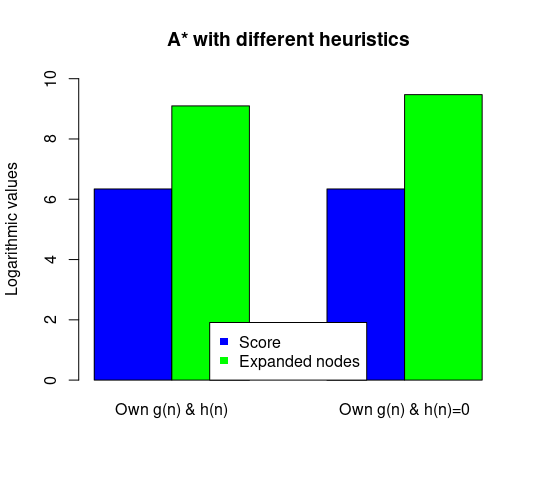
\includegraphics[scale=0.7]{q3_plot.png} 
        \caption{Comparison of A$^*$ algorithm with different heuristics in the middle layout.}
    \end{figure}
    \item The returned scores are the same with a value of 568. Using our heuristic function, the algorithm expanded 8945 nodes. While using $h(n) = 0$, the algorithm expanded 12983 nodes.
    \item The version using $h(n) = 0$ expands more nodes because using $h(n) = 0$ is equivalent of using an uninformed search algorithm which does not take into account the possible location of a goal node.
    \item A$^*$ with $h(n) = 0$ for all $n$ corresponds to the uniformed-cost search algorithm.
\end{enumerate}

\section{Experiment 2}

\begin{enumerate}[label=\alph*.,leftmargin=1.35em]
    \item Plot using natural logarithmic values:\\
    \begin{figure}[H]
        \centering
        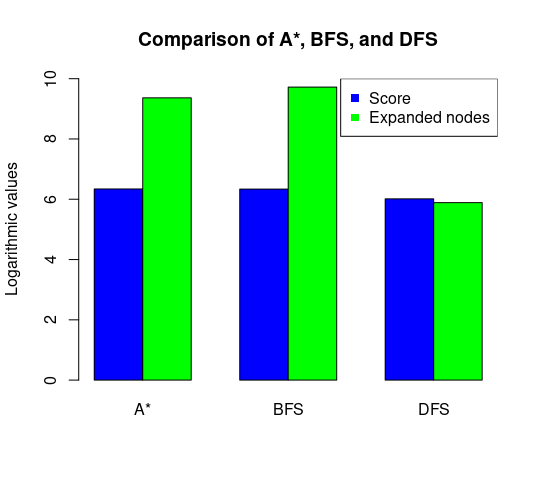
\includegraphics[scale=0.7]{q4_plot.png} 
        \caption{Comparison of the different algorithms in the middle layout.}
    \end{figure}
    \item
        \begin{itemize}
            \item A$^*$ is better than DFS in terms of score but worst when it comes to the number of expanded nodes.
            \item A$^*$ is better than BFS in terms of score and the number of expanded nodes.
        \end{itemize}
    \item These observations are due to the fact that:
        \begin{itemize}
            \item DFS is not optimal because it is going as deep as possible in the search tree until it finds a step goal which is not often the optimal but it reduces the number of expanded nodes.
            \item BFS is not optimal because it is exploring the shallowest unexplored node until it finds a step goal which is not always the optimal one. Therefore, the number of expanded nodes is high.
            \item A$^*$ is getting the best score because, as we have seen in the theoretical course, this search algorithm is optimal thanks to taking into account the cost function and the heuristic. It is taking into account the optimal path cost and the possible location of a goal node so its score is higher than the one for BFS and DFS and its number of nodes expanded is lower than the one for BFS.
        \end{itemize}
\end{enumerate}


% ==============================================================================

\end{document}

